%%% LaTeX Template
%%% This template is made for project reports
%%%	You may adjust it to your own needs/purposes
%%%
%%% Copyright: http://www.howtotex.com/
%%% Date: March 2011

%%% Preamble
\documentclass[paper=a4, fontsize=12pt]{scrartcl}	% Article class of KOMA-script with 11pt font and a4 format
\usepackage[T1]{fontenc}
\usepackage{fourier}

\usepackage[english]{babel}															% English language/hyphenation
\usepackage[protrusion=true,expansion=true]{microtype}				% Better typography
\usepackage{amsmath,amsfonts,amsthm}										% Math packages
\usepackage[pdftex]{graphicx}														% Enable pdflatex
\usepackage{url}
\usepackage{colortbl}
\usepackage{hyperref}



\usepackage{listings}
\lstset{
basicstyle=\ttfamily,
keywordstyle=\bfseries,
language=SQL,                % choose the language of the code
frame=single,	                % adds a frame around the code
aboveskip=11pt,
belowskip=11pt,
breaklines=true,                % sets automatic line breaking
breakatwhitespace=false,  % sets if automatic breaks should only happen at
showspaces=false,
showstringspaces=false
}



%%% Custom sectioning (sectsty package)
\usepackage{sectsty}												% Custom sectioning (see below)
\allsectionsfont{\centering \normalfont\scshape}	% Change font of al section commands


%%% Custom headers/footers (fancyhdr package)
\usepackage{fancyhdr}
\pagestyle{fancyplain}
\fancyhead{}														% No page header
%\fancyfoot[L]{\small \url{HowToTeX.com}}		% You may remove/edit this line 
\fancyfoot[C]{}													% Empty
\fancyfoot[R]{\thepage}									% Pagenumbering
\renewcommand{\headrulewidth}{0pt}			% Remove header underlines
\renewcommand{\footrulewidth}{0pt}				% Remove footer underlines
\setlength{\headheight}{13.6pt}


%%% Equation and float numbering
\numberwithin{equation}{section}		% Equationnumbering: section.eq#
\numberwithin{figure}{section}			% Figurenumbering: section.fig#
\numberwithin{table}{section}				% Tablenumbering: section.tab#

%%% Maketitle metadata
\newcommand{\horrule}[1]{\rule{\linewidth}{#1}} 	% Horizontal rule

\title{
		%\vspace{-1in} 	
		\usefont{OT1}{bch}{b}{n}
		%\normalfont \normalsize \textsc{University of Tuebingen} \\ [25pt]
		\horrule{0.5pt} \\[0.4cm]
		\LARGE Data Management Tool
		\horrule{2pt} \\%[0.2cm]
}
\author{
		\normalfont 								\normalsize
			Lecture: Data Management in Quanitative Biology\\					\normalsize
     		Names: Sven Fillinger, Simon Heumos, Judith Neukamm\\					\normalsize
       		 \today
}
\date{}


%%% Begin document
\begin{document}
\maketitle
%\tableofcontents

%\tableofcontents
%\vspace{2cm}
%\centerline{\bf Abstract}
%Bla bla blubb
%\noindent
%
%\newpage

\section{Introduction and Motivation}
The increasing amount of data and the participation of several institutions in a project makes it important to document well how to handle essential aspects like the storage, analysis and integration of data during the project. This can be realized with a Data Management Plan \cite{lecture}. Moreover, this plan ensures before the data collection starts that data are in correct format, well-organized and better annotated \cite{planWhy}. The documentation of the different steps throughout the data's life cycle helps other to understand and use the data in the future. 

Furthermore, the data management plan also makes the data available to other researchers upon project completion, which can impinge positive on the whole work, concerning discovery and relevance \cite{planWhy}.


There exists no standardized guidance how to create a data management plan however the DAMA Data Management Body of Knowledge \cite{DAMAInternational:2009:DGD:1593444} provides a good orientation of essential aspects which should be part of the plan \cite{lecture}. 


During the scope of the project, it was our task to develop a Data Management Planning Tool. The tool should be able to creates automatically a DMP based on an experimental design given as a .tsv file. This file was generated by \textit{QWizard} \cite{qwizard}, a portlet to input experimental data. The tool also offers users the possibility to add project information which are not included in the .tsv file.


The following chapters give an overview about the tool \textit{CMPcreator} which was implemented during the scope of this project. The last chapters compare our tool with the  already existing tool \textit{DMPTool} developed by the University of California (wie zitieren?) followed by an outlook how our tool can be extended.



%
%- based on data $\rightarrow$ description how to store, analyze, integrate data \cite{lecture}, as well as meta information\\
%- no existing standard, but DAMA-DMBOK as orientation which information are useful (!not complete!)\cite{lecture}\\
%
%- Essential aspects concern: - Data acquisition, standards, file formats  - Data sharing - Data preservation \cite{lecture}\\
%
%- why manage and share data?\\
%-- making data available $\rightarrow$ can impinge positive on the work (concerning discovery and relevance) (\url{http://libraries.mit.edu/data-management/plan/why/})\\
%- nice picture of research data life cycle: \url{http://data.library.virginia.edu/data-management/} 

\section{Experimental Design Knowledge}
On of the project's task was the implementation of results from an web-based experimental design tool called QWizard \cite{qwizard}. It is part of QBiC's web-based science gateway QPortal which handles scientific experimental projects and data. Customers are using the QWizard for setting up their experimental design and therefore provide information which already can be used for the data management plan. To name some of the information that will be available from the QWizard are detailed description of the biological entity, such as treatment or phenotype, as well as the species. Also the sample extraction is described, listing the type of tissue used as well as defined conditions used. Moreover, the QWizard will provide information of the sample size and technologies used for retrieving the data.

This information also belongs into the data management plan as it is part of the experimental design and therefore essential for the project planning and execution. We can also use the information for supporting the user during the process of generating a data management plan by suggesting storage amount and backup solutions for example.

In order to use the information given by the QWizard, we will provide an upload section, where the user can upload the file with all the content generated from QWizard and a background parser will retrieve the information as well as automatically implementing it in the report template.
\section{System Architecture}
\subsection{Java Framework}
For the setup of an own data management planning tool we decided to use the \texttt{Vaadin Framework}\footnote{\url{https://vaadin.com/home}}. \texttt{Vaadin} is a single-page web framework for Java developers that provides powerful functions for creating rich Internet applications (RIAs) without the knowledge of classical web-languages as HTML5 or CSS3. It also provides a huge library of functional components that can be included in the project and already satisfy out needs for usability and navigation.
The \texttt{Vaadin Framework} takes care of browser incompatibilities and automatically designs ajax communication protocols, which we evaluated as advantage in terms of time efficiency during the development. It is also open-source but still provides a support service. 

As we are all quite familiar with Java, the availability of a huge component library, good documentation and support as well as the capacity to build a rich Internet application convinced us to give it a chance and use it for our own creation of a data management planning tool.

\subsection{Java Application Server}
In order to run the project, local or on a web-server, we needed to set-up a Java application server. There are numerous servers available, most of them are free and open-source. For our needs, we thought it does not make a big difference which server we select as we will not use the full capacities anyway. 
Apache's Tomcat was already known to us and was used before in other projects. To get to know a new application server which also comes with a nice documentation and web interface is JBoss' Wildfly\footnote{\url{http://wildfly.org/}}. 
In our case the installation and set-up of Wildfly was easy under Linux OS. So we configured local instances on every development environment and used the server's default settings.

\subsection{Vaadin Theme}
The \texttt{Vaadin Framework} also comes with additional themes, that apply a different layout and style to the graphical interface elements. We decided to choose the theme 'Valo', as it comes with a complete set of designed components, is responsive and ensures a pleasant user experience.

\section{Result: DMPcreator}
The result of our implementation efforts is the user friendly webinterface \texttt{DMPcreator}. It enables scientists to create a data management plan based on the .tsv file produced by \texttt{QWizard}. The tool is structured into five slides. A progress bar on top of every slide gives an excellent overview of the current advances. Furthermore, the user can navigate through the slides by clicking at the buttons at the bottom on the right (present in every slide). Moreover, every slide contains a detailed description about what, where and why the user has to fill in here. Note, that every field in every slide will be parsed in the end and the information is stored in a human readable PDF file.\par
The first slide, the \textit{General Information Slide}~(figure \ref{GeneralInformationSlide}), provides fields letting the user enter general information about his project, for example the project name, the person in charge of the project and contact data. Furthermore, the user can upload his .tsv file created by \texttt{Q-Wizard}. From this uploaded data experiment details like species, experiment types, number of experiment per experiment type, and so forth are extracted for later usage (slide \textit{Storage \& Backup} (figure \ref{StorageBackupSlide}) needs this information in order to calculate required storage correctly). \par
One important topic that needs to be covered when creating a data management plan is \textit{Roles \& Responsibilities}~(figure \ref{RolesResponsibilitiesSlide}) of every project member. This second slide allows the user to assign roles to persons. The chosen values are added two a responsibilities list later being parsed by the PDF creator. \par Having specified who is responsible for which data, the user still has to decide, how the data is stored. Here steps the third slide \textit{ContentManagement} (figure \ref{ContentManagementSlide}) in. The user can assign file types to an associated description building a content. PDF creator parsed these user created contents, too. \par
How to store data efficiently is one key component in a data management plan. In the slide \textit{Storage \& Backup} (figure \ref{StorageBackupSlide}) the user is able to fill in the storage location, the RAID backup solution, the archive solution and how much data (in GB) one experiment will produce approximately. Changing the needed disk space for an experiment results in an update of the displayed total required space. So the user gets an immediate feedback when filling in necessary fields. \par
The last slide covers the topic of \textit{Dissemination} (figure \ref{Dissemination}) of data. This mask provides fields for the user to generate dissemination methods. Furthermore, by clicking on the 'Generate Report' button, the PDF creator produces the PDF. Another button ('Download Report') then allows the user to download the created report.
\begin{landscape}
	\begin{figure}[]
		\centering
		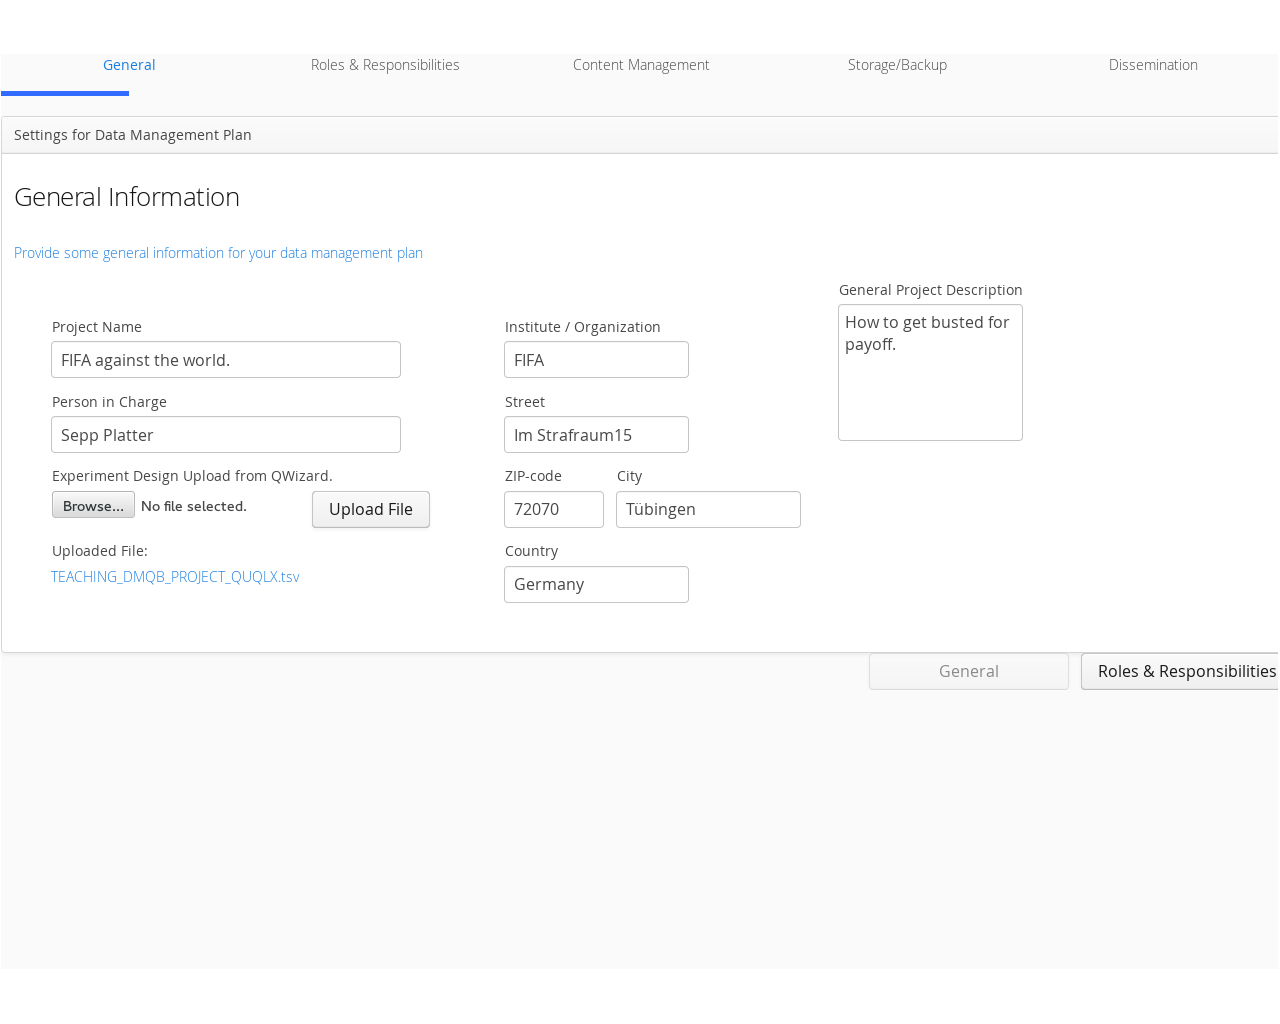
\includegraphics[width=1.2\textwidth]{pictures/GeneralInformation.png}
		\caption{\textit{General Information} Slide of \texttt{DMPcreator}. The progress bar is placed on the top. Fields that are fillable by the user can be seen below. Note, a special upload field for the .tsv file from \texttt{Q-Wizard} is visible on the left bottom.}
		\label{GeneralInformationSlide}
	\end{figure}

\begin{figure}[]
	\centering
	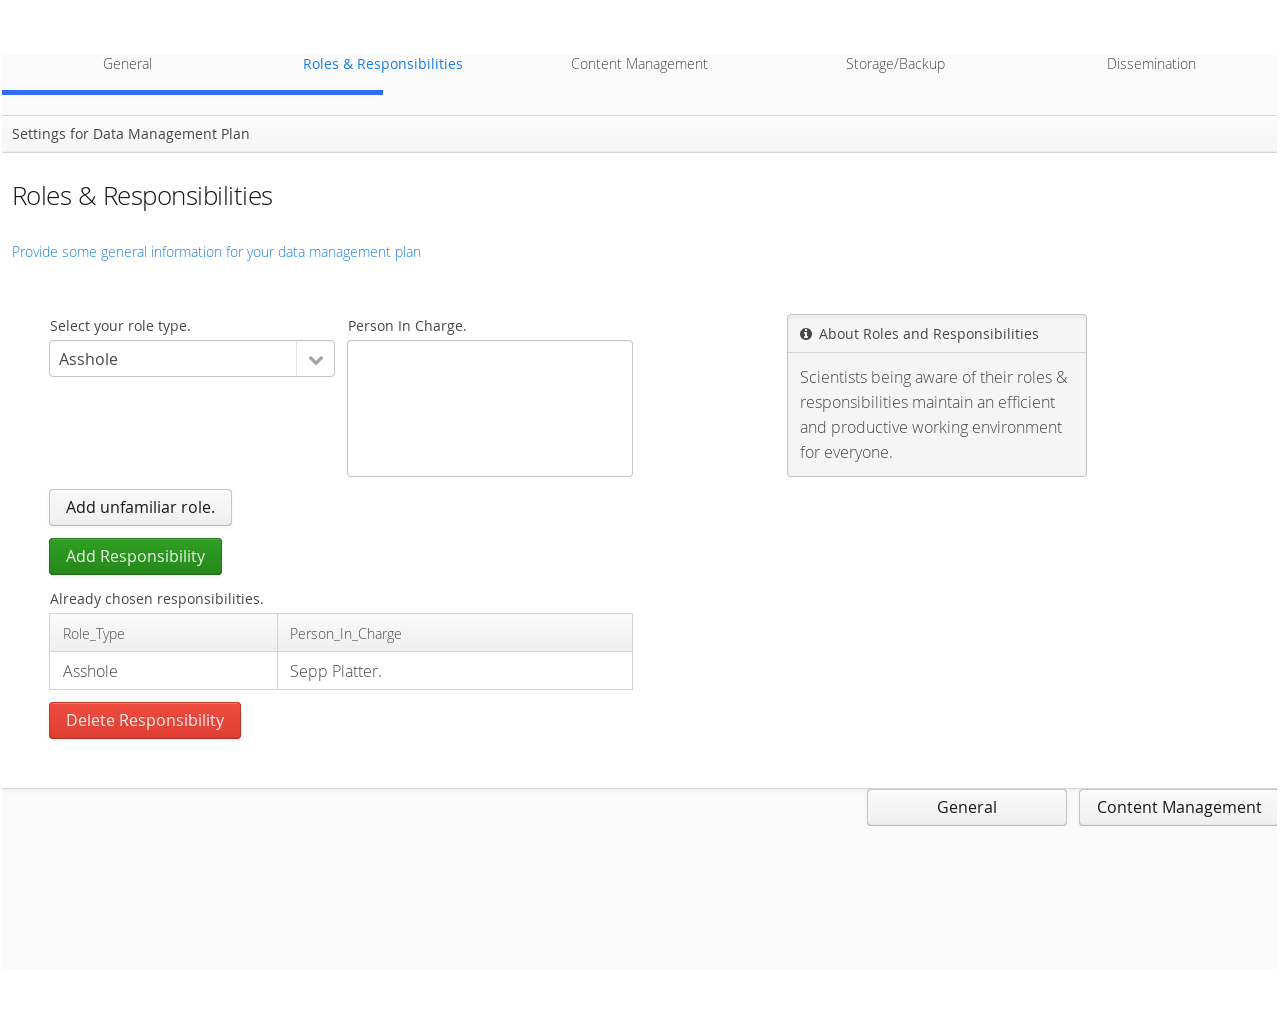
\includegraphics[width=1.2\textwidth]{pictures/RolesResponsibilities.png}
	\caption{\textit{Roles \& Responsibilities} Slide of \texttt{DMPcreator}. The progress bar is placed on the top. Fields that are fillable by the user can be seen below.}
	\label{RolesResponsibilitiesSlide}
\end{figure}

\begin{figure}[]
	\centering
	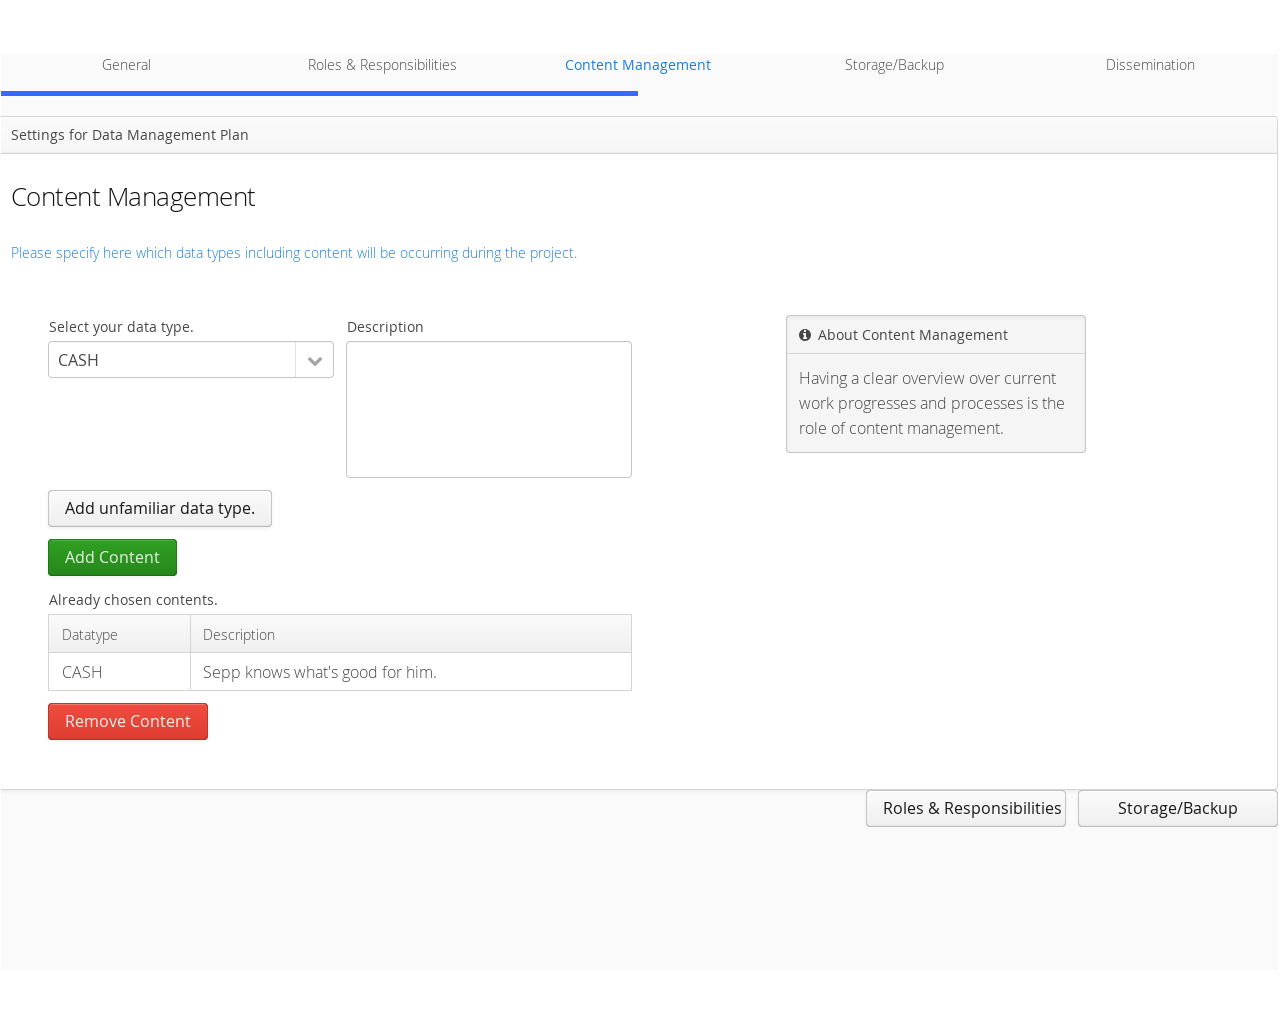
\includegraphics[width=1.2\textwidth]{pictures/ContentManagement.png}
	\caption{\textit{Content Management} Slide of \texttt{DMPcreator}. The progress bar is placed on the top. Fields that are fillable by the user can be seen below.}
	\label{ContentManagementSlide}
\end{figure}

\begin{figure}[]
	\centering
	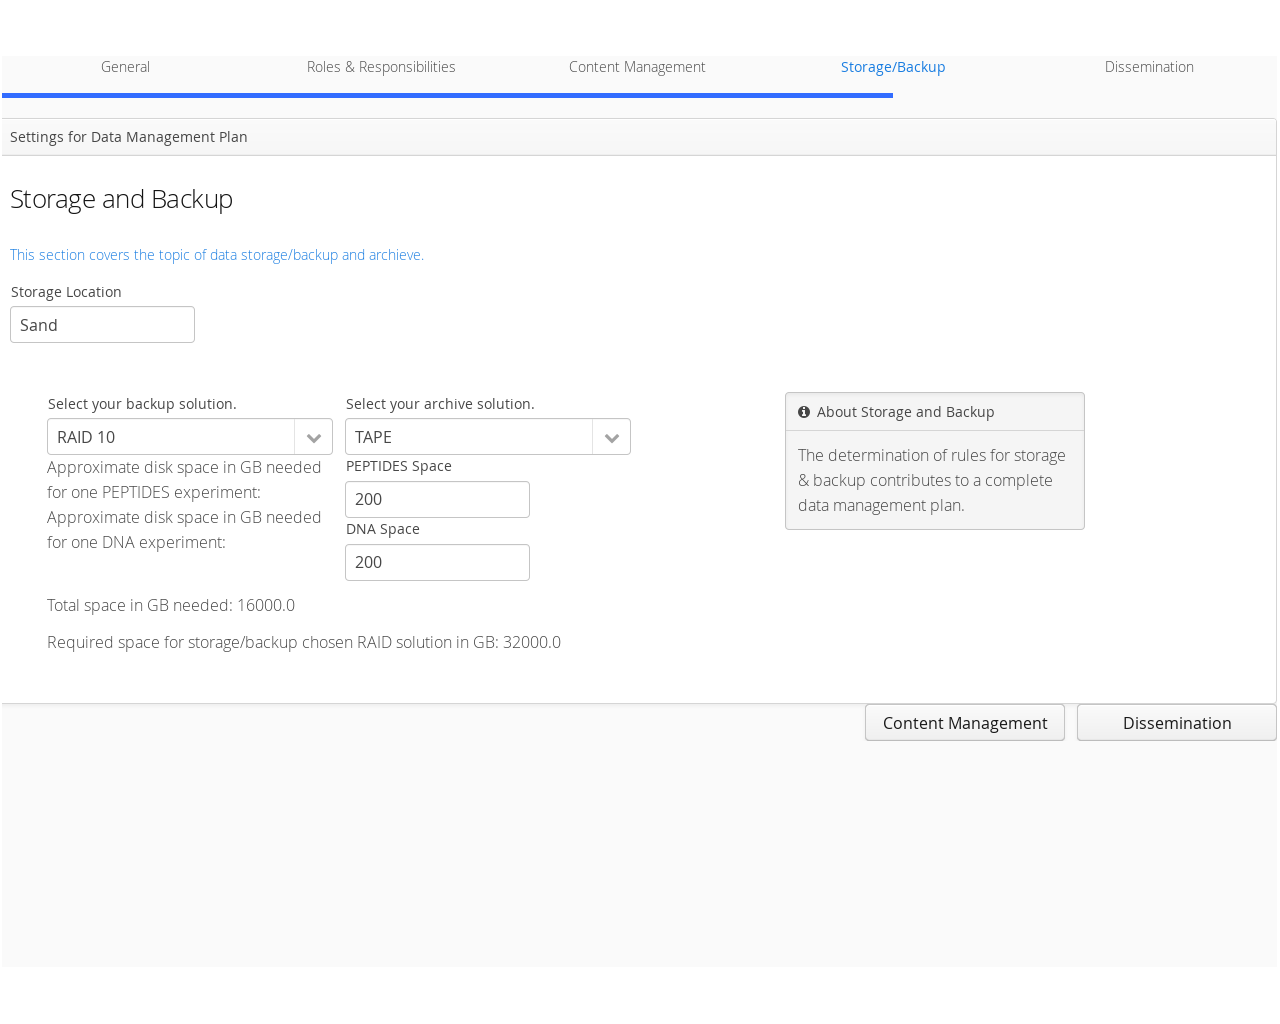
\includegraphics[width=1.2\textwidth]{pictures/StorageBackup.png}
	\caption{\textit{Storage \& Backup} Slide of \texttt{DMPcreator}. The progress bar is placed on the top. Fields that are fillable by the user can be seen below.}
		\label{StorageBackupSlide}
\end{figure}

\begin{figure}[]
	\centering
	\label{Dissemination}
	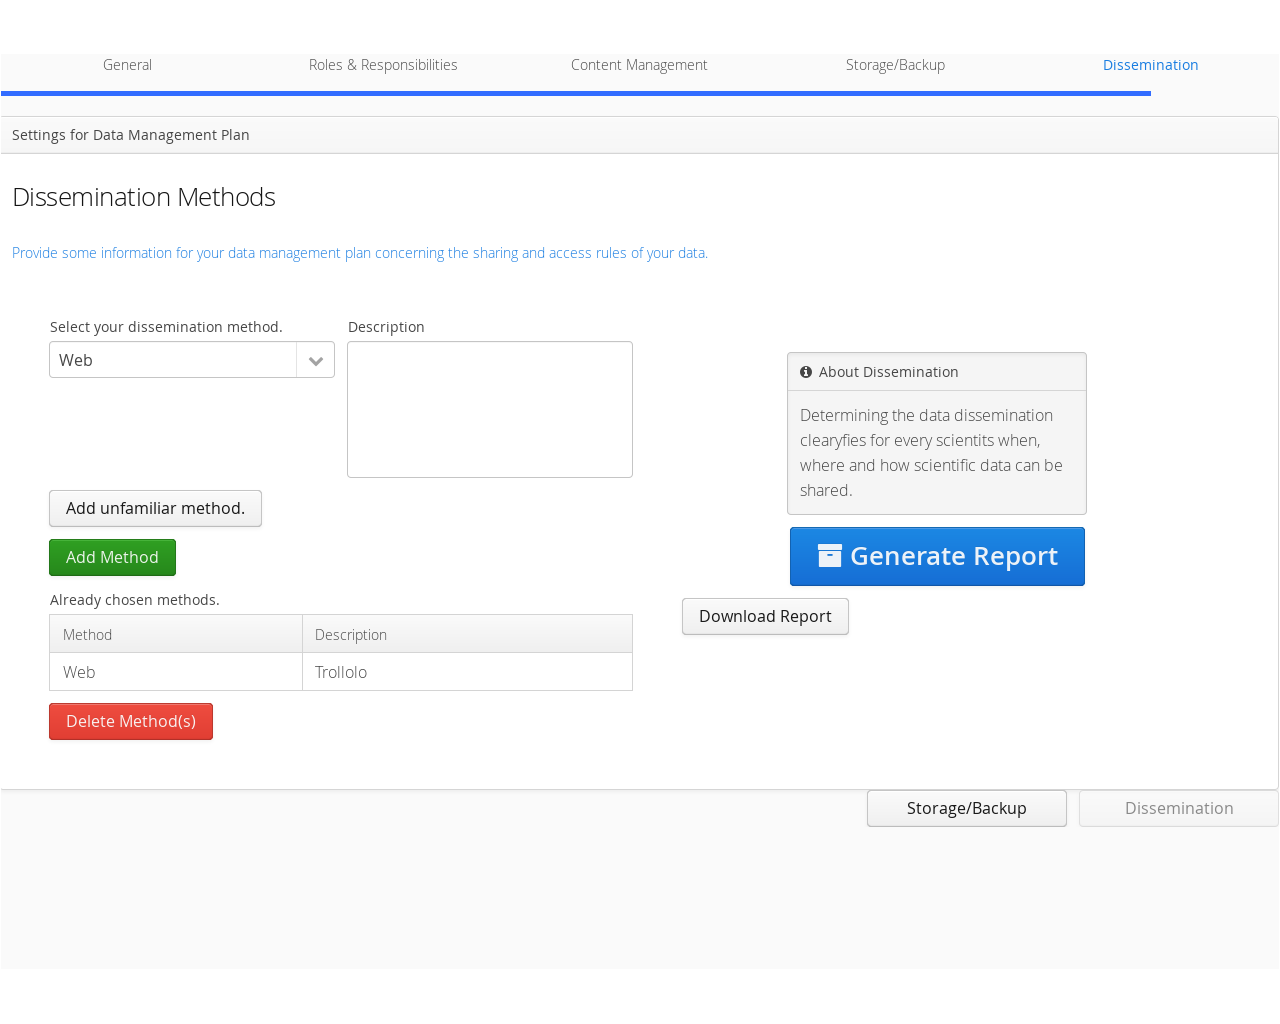
\includegraphics[width=1.2\textwidth]{pictures/Dissemination.png}
	\caption{\textit{Dissemination} Slide of \texttt{DMPcreator}. The progress bar is placed on the top. Fields that are fillable by the user can be seen below.}
\end{figure}
\end{landscape}
\section{Discussion}
Proper data management will become more and more important in the future, as new developments of technologies are going to produce an expanding amount of data. This is in particular true for scientific applications. The recent developments in next-generation sequencing and mass spectrometer analysis have shown, that there is a flood of data that is created during a project's lifetime.
Initiatives have been started over the past years, to formulate standards in data management. The DAMA International Foundation is an example for such an initiative, that took steps towards an important direction. It has defined the Data Management Book of Knowledge (DMBOK), which is a guideline for proper data management and categorizes the task in eleven different fields. 

During the lecture, we got to know the Data Management Plan Tool (DMPtool) from the University of California, which provides a guided web-interface for generating a data management plan. We experienced the tool as a step in the right direction, but remark, that it is not standardized at all, concerning the input the user can do in order to create such a plan. There are a lot of text-fields, which allow the input of free text, but this raises issues at the same time. The user can input what he wants, and there is no standard for that, nor do unexperienced user have a glue what to fill in. Though the tool provides templates, which are plans created from other users, the quality of the input varies a lot.

With our tool DMPcreator, we want to present a data management plan tool that follows the DMBOK guideline and controls some of the standards mentioned there. Additionally, we provide an integration for projects created with QWizard, a web-based experimental design tool from the Quantitative Biology Center (University of Tuebingen). The user can upload the project description as tabbed-separated file (tsv), and this content will be parsed automatically and information such as storage requirement derived from the technology type will be integrated in the web-interface as well as in the report automatically. The user can still change the input, if necessary.
The taxonomy ID in the tsv-file will be queried automatically from the NCBI web-server and translated in the organism species.
We used Vaadin as a Java framework and provide a user-friendly interface with intuitive and customizable components such as flexible drop-down menus with predefined content and dynamic tables that will display the user input. Because of the short project time, we only implemented topics from the DMBOK such as 'Storage and Backup', 'Documentation Management', 'Dissemination', 'Roles and Responsibilities' and 'General Information' for contact data. Of course, in order to provide a detailed data management plan a lot more chapters and options have to be added. We designed the software as generic as possible, developers can add more user slides and extend the class for parsing the content into the report as pdf.

We have shown, that a more user-friendly and more standardized data management plan tool is possible, and has to be the further development. The DMBOK provides the ideal template for such a tool and frameworks offer the components and functionality to build a detailed and guided interface to generate a content-rich and standardized data management plan.
\section{Outlook}

The \textit{DMPcreator} covers just a small fraction of the aspects of a data management plan. Therefore, it could be extended by adding more user slides concerning data security and data sharing for example. Furthermore, the .tsv file could be parsed more detailed. It also contains information about the experiment structure, the treatment of the individuals and the tissues, which are not yet used by generating the data management plan. 


Moreover, additional fields for user input could be added. This provides the user the possibility to create a more specific and adapted data management plan. 



\newpage
\bibliographystyle{plain}
\bibliography{cites}
%%% End document
\end{document}